% ==============================================================================
\chapter{Active Edge Assemblies}
\label{sec:activeEdgeAssemblies}
%==============================================================================    

\begin{table}[htbp]
  \centering
  \caption{Active-edge assemblies: n-in-p, produced by Advacam.}
  \label{tab:activeEdgeAssembliesList}
  \begin{tabular}{lccc}
    \toprule
    Assembly & Thickness [\micron] & Edge [\micron] \\
    \midrule
    W19\_G7 & 50 & 20-256 \\
    W19\_L8 & 50 & 20-GR257 \\
    W19\_C7 & 50 & 50-GR257 \\
    W19\_F7 & 50 & 20 G256 \\
    W5\_E2 & 100 & 50-GR GND \\
    W5\_F1 & 150 & 50-GR GND\\
    \bottomrule
  \end{tabular}
\end{table}


\begin{figure}[htbp]
  \centering
  \begin{minipage}[t]{.4\textwidth}
    \centering
    \vspace{0pt}
    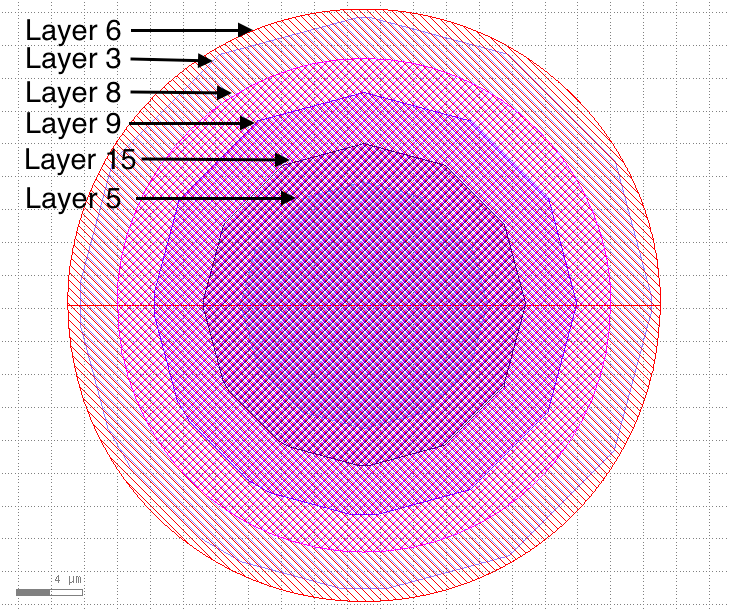
\includegraphics[width=0.95\textwidth]{figures/ActiveEdge/pixelLayout_withLayers.png}
    \caption{}
    \label{fig:PixelLayout}
  \end{minipage}
  \hfill
  \begin{minipage}[t]{.56\textwidth}
    \centering
    \vspace{0pt}
    \captionof{table}{Layers and dimensions from the gds geometry
      (taken from Timepix 20um GR FLOAT).}
    \label{tab:sources}
    \begin{tabular}{l c c}
      \toprule
      Layer number & Layer & Radius [\micron]\\
      \midrule
      6 & metal & 36 \\
      3 & - & 34.62 \\
      8 & implant & 30 \\
      9 & UBM (for thin film lift off metal) (??) & 25.6 \\
      15 & passivation & 19.5 \\
      5 & contact to connect Al to Si & 15 \\
      \bottomrule
    \end{tabular}
  \end{minipage}
\end{figure}